\documentclass{utap}

\usepackage{wrapfig}
\usepackage{verbatim}
\usepackage{fancyvrb}
\usepackage{lscape}
\usepackage{rotating}
\usepackage{xepersian}

\title{تمرین شماره‌ی ۴}
\author{ \href{mailto:zangenehsaeed412@gmail.com?subject=[AP\%20S98 A4]\%20}{سعید زنگنه},
\href{mailto:m.moridi.2009@gmail.com?subject=[AP\%20S98 A4]\%20}{محمد مریدی},
\href{mailto:sadeghian.sadaf22@gmail.com?subject=[AP\%20S98 A4]\%20}{صدف صادقیان}}
\course{برنامه‌سازی پیشرفته}
\lecturer{رامتین خسروی}
\deadline{شنبه ۲۵ اسفند ۱۳۹۷، ساعت ۲۳:۵۵}
\graphicspath{{./img/}}

\lstdefinelanguage{zabanche}{ % ino nemidoonam chie?
	morekeywords={run}
}
\lstdefinelanguage{diff}{
	morecomment=[f][\color{Black}]{---},
	morecomment=[f][\color{Red}]<,
	morecomment=[f][\color{Green}]>,
	identifierstyle=\color{Cyan},
	basicstyle=\small\ttfamily\color{Cyan},
}

\begin{document}
	\maketitle
	
	هدف از این تمرین، آشنایی شما با مفاهیم اولیه طراحی شی‌ءگرای\LTRfootnote{Object-Oriented Design} یک مسأله می‌باشد. از آنجایی که استفاده از این مفاهیم، در پیاده‌سازی سایر تمارین این درس لازم می‌باشد، پیشنهاد می‌شود به این پروژه زمان کافی را اختصاص دهید.
	\section{مقدمه}
	
	\hspace{5mm}
همانطور که می‌دانید، پردازنده‌\LTRfootnote{Processor}ای با یک واحد پردازشی\LTRfootnote{Processing Unit}، در یک زمان مشخص نمی‌تواند بیشتر از یک کار را انجام دهد؛ این عبارت بدین معنا می‌باشد که وقتی دستورات\LTRfootnote{Instructions} مربوط به یک برنامه\LTRfootnote{Program} بر روی پردازنده در حال اجرا می‌باشد، این امکان وجود ندارد که دستورات مربوط به برنامه‌ای دیگر نیز به طور همزمان بر روی همان پردازنده در حال اجرا باشد. اما همه ما می‌دانیم که در این پردازنده‌ها نیز، می‌توان چندین برنامه را به صورت هم‌روند\LTRfootnote{Concurrent} اجرا کرد. اجرای هم روند با اجرای موازی \LTRfootnote{Parallel} متفاوت می‌باشد. وقتی دو برنامه به صورت موازی اجرا می‌شوند، بدین معنا می‌باشد که هر دو برنامه در زمانی مشخص بطور همزمان در حال اجرا می‌باشند. اما اصطلاح هم‌روندی، به معنی به اشتراک گذاری زمان \LTRfootnote{Time-Sharing} می‌باشد که این احساس را بوجود می‌آورد که هر دو برنامه به طور همزمان اجرا می‌شوند. اشتراک‌گذاری زمان برای دو برنامه بدین صورت می‌باشد که پردازنده به مدت زمان \LR{t\textsubscript{1}} در اختیار برنامه اول قرار می‌گیرد و سپس به مدت زمان  \LR{t\textsubscript{2}} در اختیار برنامه دوم قرار می‌گیرد. پس از آن دوباره برنامه اول پردازنده را در اختیار گرفته و این چرخه تا پایان یکی از دو برنامه ادامه پیدا می‌کند. بدین ترتیب اگر  \LR{t\textsubscript{1}} و  \LR{t\textsubscript{2}} به اندازه کافی کوچک اختیار شوند، این احساس به کاربر القا می‌شود که هر دو برنامه به طور همزمان در حال اجرا می‌باشند.
	
	\section{پیش زمینه}
		\subsection{پردازنده‌ی چندهسته‌ای\protect\LTRfootnote{Multicore Processor}} % [leftmargin=6em]
		\hspace{5mm}
پردازنده چند‌هسته‌ای یک مولفه محاسباتی \LTRfootnote{Computing Component} می‌باشد که از دو یا تعداد بیشتری واحد پردازشی به نام هسته\LTRfootnote{Core} تشکیل شده است. یک هسته، وظیفه اجرای دستورات یک برنامه را بر عهده دارد. در این پردازنده، این امکان وجود دارد که چندین دستور بطور همزمان بر روی هسته‌های مختلف و به صورت موازی اجرا شوند.
		\begin{figure}[H]
			\centering
			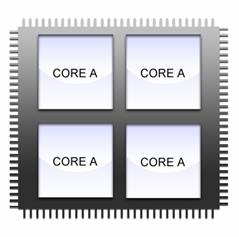
\includegraphics[width=0.30 \textwidth]{MultiCore.jpg}     
		\end{figure}
	
		\subsection{پردازه\protect\LTRfootnote{Process}} % [leftmargin=6em]
		\hspace{5mm}
	یک پردازه نمونه‌ای از یک برنامه می‌باشد که داخل حافظه\LTRfootnote{Memory} بارگذاری\LTRfootnote{Load} شده است و در حال اجرا می‌باشد. برای مثال زمانی که شما برنامه‌ خود را کامپایل می‌کنید، کامپایلر یک فایل اجرایی متناظر با کد شما ایجاد می‌کند که شامل کد قابل فهم برای ماشین شما می‌باشد. زمانی که شما این فایل اجرایی را با استفاده رابط خط فرمان\LTRfootnote{Command-Line Interface} (و یا به هر صورت دیگری) اجرا می‌کنید،‌ سیستم‌عامل\LTRfootnote{Operating System} به برنامه شما، منابع\LTRfootnote{Resources} لازم را اختصاص داده و آن را در حافظه اصلی بارگذاری می‌کند که به آن پردازه گفته می‌شود.

		\subsection{ریسه\protect\LTRfootnote{Process}} % [leftmargin=6em]	
		\hspace{5mm}
	در علم کامپیوتر، ریسه‌ای از اجرا، کوچکترین دنباله‌ای از دستورات می‌باشد که می‌توانند به‌طور مجزا، مدیریت و برنامه‌ریزی شوند. در حالت کلی، مجموعه‌ای از ریسه‌ها، یک پردازه را تشکیل داده و این ریسه‌‌ها می‌توانند بصورت هم‌روند اجرا شوند.
	
%	    \begin{figure}[H]
%	    	\centering
%	    	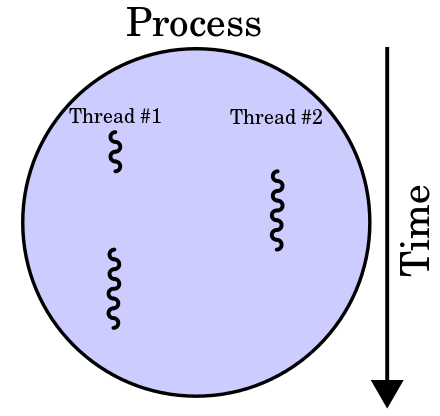
\includegraphics[width=0.15 \textwidth]{Multithreaded_process.png}     
%	    \end{figure}
    
    	\subsection{برنامه‌ریز\protect\LTRfootnote{Scheduler}} % [leftmargin=6em]
    	\hspace{5mm}
    برنامه‌ریزی\LTRfootnote{Scheduling} در سطح ریسه‌‌ها، بدین معنا می‌باشد که به هر کدام از ریسه‌ها، منابع لازم -که در برنامه‌ی شما، هسته‌های در حال برنامه‌ریزی است - برای انجام کامل کار خود اختصاص داده شود. رویکردهای گوناگونی برای نحوه اختصاص منابع به ریسه‌ها وجود دارد که در این تمرین، با یک نوع از آن که جلوتر توضیح داده خواهد شد، آشنا می‌شوید.
    	\subsection{برنامه‌ریز دوره‌ای} % [leftmargin=6em]
    	\hspace{5mm}
    	ایده اصلی برنامه‌ریز دوره‌ای \LTRfootnote{Round-Robin Scheduler} بدین صورت می‌باشد که برنامه‌ریز، به هر ریسه بازه زمانی معینی را اختصاص می‌دهد و منابع مورد نیاز آن را تأمین می‌کند. تخصیص منابع در ابتدای بازه انجام می‌شود و انتهای بازه نیز منابع پس گرفته می‌شود. به این بازه زمانی که منابع در اختیار یک ریسه می‌باشد، یک برش زمانی\LTRfootnote{Time Slice} گفته می‌شود.
    	در این روش، به هر ریسه عددی تحت عنوان \textbf{تعداد برش‌های زمانی} که برای انجام کار خود نیاز دارد، نسبت داده می‌شود. این عدد، بیان‌‌کننده تعداد بازه‌های زمانی می‌باشد که برنامه‌ریز، منابع را به این ریسه اختصاص می‌دهد.
    	در پیاده‌سازی این روش، یک صف از ریسه‌‌ها به ازای هر هسته در نظر گرفته می‌شود. عملیات برنامه‌ریزی بدین صورت انجام می‌شود که منابع از ریسه‌ای که بر روی هسته در حال اجرا بوده است(ریسه ابتدای صف)، گرفته شده و در صورتی که تعداد برش‌های زمانی این ریسه به پایان نرسیده باشد، به انتهای صف اضافه می‌شود (در صورت اتمام برش‌های زمانی، از صف برنامه‌ریزی حذف می‌شود). سپس منابع لازم، به ریسه‌ای که در ابتدای صف وجود دارد تخصیص داده می‌شود.
    	\newline
    	برای مثال فرض کنید یک هسته داریم که در صف آن به ترتیب ریسه‌ A با تعداد ۲ برش زمانی، ریسه‌ B با ۱ برش زمانی و ریسه C با ۱ برش زمانی قرار دارند. در روش برنامه‌ ریز دوره‌ای در این هسته ابتدا یک برش زمانی از ریسه A اجرا می‌شود، سپس این ریسه به انتها‌ی صف منتقل می‌شود، در ادامه یک برش زمانی از ریسه  ‌B و سپس یک برش زمانی از ریسه C اجرا می‌شود. چون اجرا ریسه های B و C تمام شده است حال فقط ریسه A در صف باقی مانده‌است و در نهایت یک برش زمانی از ریسه A اجرا می‌شود تا دیگر ریسه‌ای در صف هسته باقی‌ نماند.
    	
	\section{شرح تمرین}
	\hspace{5mm}
	در این تمرین، شما به پیاده‌سازی یک برنامه‌ریز دوره‌ای می‌پردازید. این برنامه‌ریز باید این توانایی را داشته باشد که هنگامی که پردازه‌ای به سیستم اضافه شد، ریسه‌های مربوط به این پردازه را بین هسته‌های پردازنده، به صورت متعادل توزیع کند. دستوراتی که برنامه شما باید از طریق \textbf{جریان ورودی استاندارد\LTRfootnote{Standard Input Stream}} گرفته و پردازش کند در ادامه‌ی شرح تمرین آمده است.
	
	\begin{figure}[H]
		\centering
		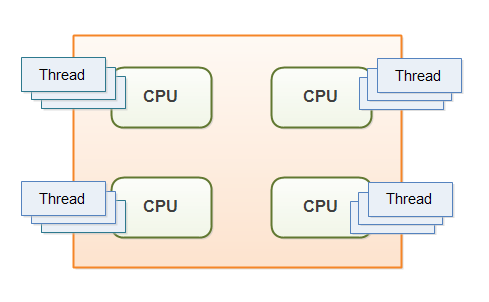
\includegraphics[width=0.5 \textwidth]{ThreadsOnCore.png}     
	\end{figure}
	
	
	\subsection{اضافه‌کردن یک هسته به هسته‌های قابل برنامه‌ریزی}
	\hspace{5mm}
	این دستور، یک هسته به هسته‌های قابل برنامه‌ریزی توسط برنامه‌ریز می‌افزاید. هر هسته دارای عددی یکتا، بعنوان شماره هسته می‌باشد که برنامه‌ی شما باید آن را خودکار و به طور افزاینده از عدد ۱به هسته‌ها اختصاص دهد.

	 \linespread{1.6}
	\begin{latin}%
		\centering
		\begin{minipage}[t]{1\textwidth}
			{\VerbatimInput[frame=lines,label={\rl{دستور ورودی}}]{add_core_in.txt}}
			{\VerbatimInput[frame=lines,label={\rl{خروجی}}]{add_core_out.txt}}
		\end{minipage}%
	\end{latin}
	
	\subsection{اضافه‌کردن یک پردازه}
	\hspace{5mm}
	با اجرای این دستور، یک پردازه به پردازه‌های تحت برنامه ریزی اضافه‌ شده و به آن شماره‌ا‌‌ی یکتا نسبت داده می‌شود. دومین آرگومان این دستور، تعداد ریسه‌های آن پردازه بوده و آرگومان‌‌های بعدی، به ازای هر ریسه تعداد برش‌های زمانی مورد نیاز آن ریسه را تعیین می‌کند. دقت کنید شماره‌‌ها‌ی یکتایی که به ریسه‌های یک پردازه نسبت می‌دهید باید از ۱ شروع شوند. برای اختصاص دادن ریسه ‌های یک پردازه به هسته‌ها، به ترتیب از اولین ریسه شروع کرده و هر ریسه را به اولین هسته‌ای  که تعداد ریسه‌های کمتری در صف خود دارد اختصاص می‌دهیم.
	
	\linespread{1.6}
	\begin{latin}%
		\centering
		\begin{minipage}[t]{1\textwidth}
			{\VerbatimInput[frame=lines,label={\rl{دستور ورودی}}]
			{add_process_in.txt}}
			{\VerbatimInput[frame=lines,label={\rl{خروجی}}]
			{add_process_out.txt}}
			{\VerbatimInput[frame=lines,label={\rl{نمونه ورودی}}]
			{add_process_in_sample.txt}}
		\end{minipage}%
	\end{latin}

	\subsection{نمایش وضعیت هسته‌ها}
	\hspace{5mm}
	کاربر با اجرای دستور زیر می‌تواند وضعیت تمام هسته‌های موجود در برنامه‌ریز و ریسه‌های درون صف هر هسته را مشاهده کند. در صورتی که صف یک هسته‌ خالی بود نیز اطلاعاتش باید در خروجی بیاید.
	
	\linespread{1.6}
	\begin{latin}%
		\centering
		\begin{minipage}[t]{1\textwidth}
			{\VerbatimInput[frame=lines,label={\rl{دستور ورودی}}]
				{show_cores_stat_in.txt}}
			{\VerbatimInput[frame=lines,label={\rl{خروجی به ازای هر هسته}}]
			{show_cores_stat_out.txt}}
			{\VerbatimInput[frame=lines,label={\rl{خروجی نمونه}}]
				{sample_show_cores_stat_out.txt}}
		\end{minipage}%
	\end{latin}

	\subsection{فعالسازی هسته‌ها}
	\hspace{5mm}
	در هر لحظه از اجرای برنامه، کاربر می‌تواند با وارد کردن این دستور، تمام هسته‌ها را برای مدت یک برش زمانی اجرا کند. اجرای هسته به این معنا می‌باشد که یک ریسه‌ را از ابتدای صف خود  اجرا کرده و یک واحد از برش‌های زمانی آن می‌کاهد. بعد از بررسی غیر صفر بودن برش‌های زمانی آن، ریسه را به انتهای صف اضافه می‌کند (توجه شود که در صورت صفر شدن این مقدار،‌ ریسه باید از صف هسته حذف شود).
	خروجی این دستور نیز، شماره پردازه و شماره ریسه‌هایی است که در هر هسته اجرا شده است. اگر در یک برش زمانی صف یک هسته خالی بود نام این هسته\textbf{ نباید} در خروجی آن برش زمانی باشد.
	
	\linespread{1.6}
	\begin{latin}%
		\centering
		\begin{minipage}[t]{1\textwidth}
			{\VerbatimInput[frame=lines,label={\rl{دستور ورودی}}]
				{run_cores_in.txt}}
			{\VerbatimInput[frame=lines,label={\rl{خروجی به ازای هر هسته}}]
				{run_cores_out.txt}}
			{\VerbatimInput[frame=lines,label={\rl{نمونه خروجی }}]
				{run_cores_out_sample.txt}}
		\end{minipage}%
	\end{latin}

	\subsection{اتمام کار تمام ریسه‌های موجود}
	\hspace{5mm}
	در هر لحظه از اجرای برنامه، کاربر می‌تواند با وارد کردن این دستور، تمام هسته‌ها را تا اتمام کار تمامی ریسه‌های موجود در صف‌ها‌ی هسته‌ها فعال کند.
	خروجی این دستور نیز به ازای هر برش زمانی، مانند دستور فعالسازی یک هسته است. اگر در یک برش زمانی صف یک هسته خالی بود نام این هسته نباید در خروجی آن برش زمانی باشد. عدد برش‌های زمانی نیز در هر بار اجرای این دستور از عدد ۱ شروع می‌شود.
	
	\linespread{1.6}
	\begin{latin}%
		\centering
		\begin{minipage}[t]{1\textwidth}
			{\VerbatimInput[frame=lines,label={\rl{دستور ورودی}}]
				{finish_tasks_in.txt}}
			{\VerbatimInput[frame=lines,label={\rl{خروجی}}]
				{finish_tasks_out.txt}}
		\end{minipage}%
	\end{latin}
	
	\section{نکات تکمیلی}
	\hspace{5mm}
	در این تمرین، اختصاص عددی یکتا به یک موجودیت‌\LTRfootnote{Entity}،‌ بدین صورت می‌باشد که مقدار اولیه عددی که به موجودیت‌ها تخصیص داده می‌شود، برابر با \textbf{یک} بوده و با اضافه شدن هر موجودیت، یک واحد به این شمارنده افزوده می‌شود.
	
	\section{نحوه‌ی تحویل}
	\hspace{5mm}
	تمام فایل‌های برنامه‌ی خود را در قالب یک فایل با پسوند \textbf{zip} و نام \lr{A4-SID.zip} در صفحه‌ی \lr{CECM} درس بارگذاری کنید که \lr{SID} شماره‌ی دانشجویی شماست؛ برای مثال اگر شماره‌ی دانشجویی شما ۸۱۰۱۹۷۹۹۹ باشد، نام پرونده‌ی شما باید \lr{A4-810197999.zip} باشد. 
	\newline
	برای اطمینان از درستی قالب فایل آپلودی خود، اسکریپتی در صفحه درس بارگذاری شده است را در کنار فایل خود قرار دهید و دستور
	\lr{./test A4-SID.zip}
	را اجرا کنید. دقت کنید خروجی این دستور باید اختلاف خروجی برنامه شما با خروجی مورد انتظار از برنامه(که درصورت پیاده‌سازی صحیح، نباید خروجی نشان داده شود) را نشان دهد و هر خروجی دیگری غیرقابل قبول می‌باشد.
	\begin{itemize}
		\item برنامه‌ی شما باید در سیستم‌عامل لینوکس و با مترجم \lr{g++} با استاندارد \lr{\texttt{c++11}} ترجمه و در زمان معقول برای ورودی‌های آزمون اجرا شود.
		\item از صحت قالب\LTRfootnote{Format} ورودی‌ها و خروجی‌های برنامه‌ی خود مطمئن شوید.
		\item با توجه با این که این اولین پروژه‌ی \lr{Multifile} شماست به این نکته توجه داشته باشید که برای ساخت\LTRfootnote{Build} برنامه‌ی خود حتما از \lr{Makefile} استفاده کنید و فایل اجرایی نهایی شما اسم \lr{Scheduler.out} را داشته باشد. در صورت عدم رعایت این نکات نمره‌ای از آزمون‌های خودکار ورودی و خروجی به شما تعلق نخواهد گرفت.
		\item رعایت سبک برنامه‌نویسی درست، تمیز~بودن برنامه‌ی شما و طراحی درست ساختار‌های داده‌ی شما در نمره‌ی تمرین تأثیر زیادی دارد.
		\item هدف این تمرین یادگیری شماست. لطفاً تمرین را خودتان انجام دهید. در صورت کشف تقلب مطابق قوانین درس با آن برخورد خواهد شد.
	\end{itemize}
	
	
	%%%%%%%%%%%%%%%%%%%%%%%%%%%%%%%%%%%%%%%%%%%%%%%%%%%%%%%%%%%%%%%%%%%%%%%%%%%%%%%%%%%%%%%%%%%%%%%%%%%%%%%%%%%%%%%%%%%%%%%%%%%%%
\end{document}